\documentclass[11pt]{article}
\usepackage[BoldFont,SlantFont,CJKchecksingle]{xeCJK}
\usepackage[top=0.5in,bottom=0.5in,left=1.25in,right=0.8in]{geometry}
\setCJKmainfont[BoldFont=SimHei]{SimSun}
\setCJKmonofont{SimSun}% 设置缺省中文字体
\parindent 0em   %段首缩进
%\usepackage{indentfirst}	%设置第一段也首行缩进
\linespread{1}	%设置行距
\addtolength{\parskip}{.4em}	%增加段间距0.4em
\usepackage{amsmath} % 插入数学公式
\usepackage[colorlinks,linkcolor=blue]{hyperref} 	%设置超链接

% 设置页眉页脚
\usepackage{fancyhdr}
\pagestyle{fancy}
\lhead{} 
\chead{} 
\rhead{\bfseries {ramayzhu0625@gmail.com}} 
\lfoot{} 
\cfoot{}
\rfoot{\thepage} 
\renewcommand{\headrulewidth}{0.4pt} 
\renewcommand{\footrulewidth}{0.4pt}

% \includegraphics[width = .8\textwidth]{pic.png}  图片的宽度会被缩放至页面宽度的百分之八十,图片的总高度会按比例缩放 

\begin{document}
	\title{Machine Learning Week-5}
	\author{ramay7}
	
	\maketitle % 显示标题
	\tableofcontents % 生成目录
	%\newpage
	
	\section{Hypothesis}
		Logistic regression:
		$$\min \limits_{\theta} -\frac{1}{m}\left[ \sum_{i=1}^{m} y^{(i)} \log(h_{\theta}(x^{(i)})) + (1-y^{(i)})\log (1-h_{\theta}(x^{(i)})) \right] + \frac{\lambda}{2m}\sum_{j=1}^{n} \theta_{j}^2$$
		support vector machine hypothesis:
		$$\min \limits_{\theta} C \left[ \sum_{i=1}^{m} y^{(i)} cost_{1}(\theta ^ T x^{(i)}) + (1-y^{(i)})cost_{0}(\theta ^ T x^{(i)}) \right] + \frac{1}{2}\sum_{j=1}^{n} \theta_{j}^2$$
		for some obvious reason, we can know: $C = \frac{1}{\lambda}$
	\section{SVM Decision Boundary}
		Then the next two picturs show the curve of logistic function while in the case of y = 1 and y = 0:
		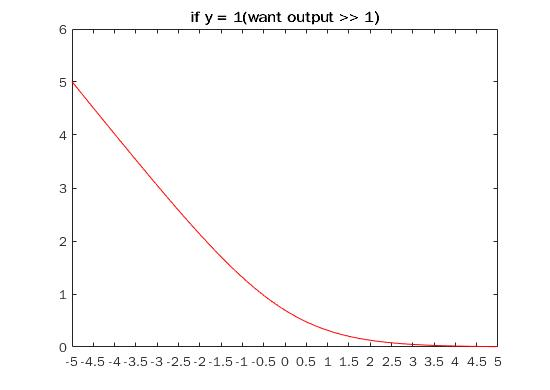
\includegraphics[width=3.5in]{if_y_=_1}
		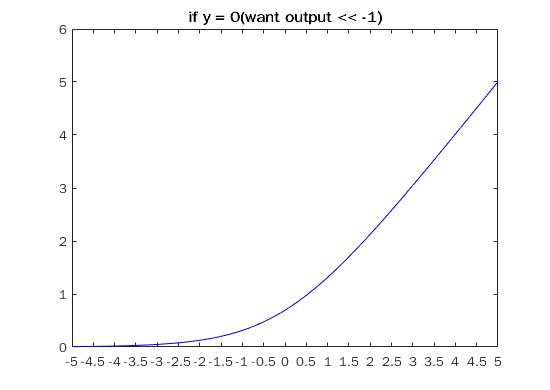
\includegraphics[width=3.5in]{if_y_=_0}
		So we can simplify the hypothesis as:
		$$
		\min \limits_{\theta}\frac{1}{2} \sum_{j=1}^{n}\theta_{j}^2
		$$
		Due to the fact that $\theta ^ T x^{(i)} \geq 1$ if $y^{(i)} = 1$ and $\theta ^ T x^{(i)} \leq -1$ if $y^{(i)} = 0$.
	\section{Kernels and Similarity}
		$$f_1=similarity(x, l^{(1)}) = \exp(-\frac{|| x- l^{(1)}|| ^2}{2\delta ^ 2})$$
		If $x\approx l^{(1)}, f_1 = 1$; If $x$ is far from $l^{(1)}$, $f_1=0$.
	\section{SVM Parameters}
		$C(=\frac{1}{\lambda})$.
		\begin{itemize}
			\item Large C: Lower bias, high variance
			\item Small C: Higher bias, low variance
		\end{itemize}
		$\delta ^ 2$:
		\begin{itemize}
			\item Large $\delta ^ 2$: Feature $f_i$ vary more smoothly; Higher bias, lower variance
			\item Small $\delta ^ 2$: Feature $f_i$ vary less smoothly; Lower bias, higher variance
		\end{itemize}
	\section{Logistic Regression vs SVMs}
		n = number of features, m = number of training examples
		If n is large(relative to m):
		\begin{itemize}
			\item use logistic regression, or SVM without a kernel("linear kernel")
		\end{itemize}
		If n is small, m is intermediate:
		\begin{itemize}
			\item use SVM with Gaussian Kernel
		\end{itemize}
		If n is small, m is large:
		\begin{itemize}
			\item Create/add more features, then use logistic regression or SVM withut a kernel
		\end{itemize}
		
		Neural network is likely to work well for most of these settings, but may be slower to train.
\end{document}